\documentclass[12pt]{article}
\usepackage[
  top=2.50cm,
  bottom=1.50cm,
  left=1.50cm,
  right=1.50cm
]{geometry} 
\usepackage{amsmath,amsthm,amssymb}
\usepackage{algorithm,algorithmic}
\usepackage{graphicx}
\usepackage{tikz}

\newenvironment{theorem}[2][Theorem]{\begin{trivlist}
\item[\hskip \labelsep {\bfseries #1}\hskip \labelsep {\bfseries #2.}]}{\end{trivlist}}
\newenvironment{lemma}[2][Lemma]{\begin{trivlist}
\item[\hskip \labelsep {\bfseries #1}\hskip \labelsep {\bfseries #2.}]}{\end{trivlist}}
\newenvironment{exercise}[2][Exercise]{\begin{trivlist}
\item[\hskip \labelsep {\bfseries #1}\hskip \labelsep {\bfseries #2.}]}{\end{trivlist}}
\newenvironment{problem}[2][Problem]{\begin{trivlist}
\item[\hskip \labelsep {\bfseries #1}\hskip \labelsep {\bfseries #2.}]}{\end{trivlist}}
\newenvironment{question}[2][Question]{\begin{trivlist}
\item[\hskip \labelsep {\bfseries #1}\hskip \labelsep {\bfseries #2.}]}{\end{trivlist}}
\newenvironment{corollary}[2][Corollary]{\begin{trivlist}
\item[\hskip \labelsep {\bfseries #1}\hskip \labelsep {\bfseries #2.}]}{\end{trivlist}}

\begin{document}

\title{Homework 4}
\author{Thomas Kim~tsk389~51835\\David Munoz~dam2989~51840\\
CS331 Algorithms and Complexity}

\renewcommand{\arraystretch}{2.0}

\date{} % Suppress the datn{minipage}{0.5\textwidth}

% ------------------
% Begin Cover Page
% ------------------

\maketitle
% ------------------
% Begin Homework
% ------------------

\onecolumn

\begin{problem}
    {Q1: 13.2}
    Consider a county in which 100,000 people vote in an election.
    There are only two candidates on the ballot: a Democratic candidate (denoted $D$) and
    and Republican candidate $R$. As it happens, this county is heavily Democratic, so 80,000
    people go to the polls with the intention of voting for $D$, and 20,000 go to the polls with the intention of voting for $R$.\\

    However, the layout of the ballot is a little confusing, so each voter, independently and with probability $\frac{1}{100}$, votes for the
    wrong candidate - that is, the one that he or she \textit{didn't} intend to vote for.
    (Remember that in this election, there are only two candidates on the ballot.)\\

    Let $X$ denote the random variable equal to the number of votes received by the Democratic candidate $D$ when the voting is conducted with this
    process of error. Determine the expected value of $X$, and give an explanation of your derivation of this value.
\end{problem}

\begin{problem}
    {Q2}
    Is the set of rational numbers countably infinite or uncountably infinite? \\
    \textbf{Countably Infinite} \\
    \begin{proof}
        Let $r \in \mathbb{Q}$ be a rational number. \\
        Consider rational numbers of the form $\frac{a}{b}$ where $a \in \mathbb{Z} \land b \in \mathbb{Z}_{\geq 0} \land gcd(a,b) = 1$ \\
        Claim: All rational numbers $\frac{q}{r}, q, r \in \mathbb{Z}$ can be expressed in this form. \\
        First, factor out $-1$ from all negative $q, r$, such that the number is expressed $s\frac{|q|}{|r|}$ where $s = (-1)^1 \lor s = (-1)^2$ \\
        Next, divide $q, r$ by $gcd(q, r)$ such that the number is expressed $s \frac{|q'|}{|r'|}$ where $q', r'$ are the result after dividing $q, r$ by $gcd(q, r)$ \\
        By the definition of gcd, $q', r'$ share no common prime factors \\
        Now, define a mapping $f: \mathbb{Q} \rightarrow \mathbb{Z} \times \mathbb{N}$ as follows: \\
        $f(\frac{a, b}) = (a, b)$ \\
        This mapping is clearly onto, as every Cartesian pair can be mapped to a corresponding real number by taking $(a,b) \rightarrow \frac{a}{b}$ \\
        The cartesian product of $\mathbb{Z} \times \mathbb{N}$ is countably infinite \\
        Therefore, the rational numbers are countably infinite. \\
    \end{proof}
\end{problem}

\begin{problem}
  {Q3(a)}
  ~\\
  \begin{center}
    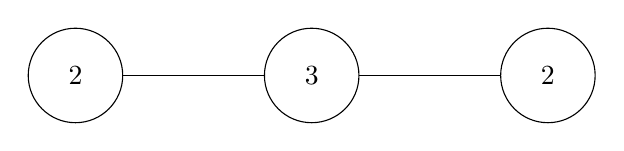
\begin{tikzpicture}[scale=0.2]
      \tikzstyle{every node}+=[inner sep=0pt]
      \draw [black] (5,0) circle (3);
      \draw (5,0) node {$2$};
      \draw [black] (20,0) circle (3);
      \draw (20,0) node {$3$};
      \draw [black] (35,0) circle (3);
      \draw [black] (35,0) node {$2$};
      \draw [black] (23,0) -- (32,0);
      \draw [black] (8,0) -- (17,0);
    \end{tikzpicture}
  \end{center}
  In this example, the middle node will be chosen and the two side nodes discarded for a total weight of $3$. \\
  If the middle node was discarded and the two side nodes chosen, the total weight would have been $4 > 3$. \\
\end{problem}

\begin{problem}
  {Q3(b)}
  ~\\
  \begin{center}
    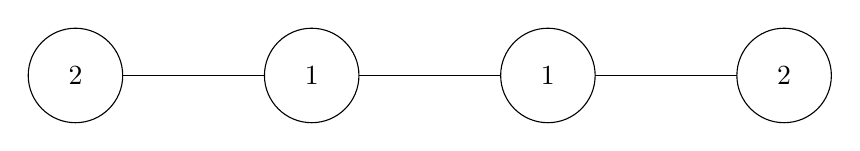
\begin{tikzpicture}[scale=0.2]
      \tikzstyle{every node}+=[inner sep=0pt]
      \draw [black] (5,0) circle (3);
      \draw (5,0) node {$2$};
      \draw [black] (20,0) circle (3);
      \draw (20,0) node {$1$};
      \draw [black] (35,0) circle (3);
      \draw (35,0) node {$1$};
      \draw [black] (50,0) circle (3);
      \draw (50,0) node {$2$};
      \draw [black] (8,0) -- (17,0);
      \draw [black] (23,0) -- (32,0);
      \draw [black] (38,0) -- (47,0);
    \end{tikzpicture}
  \end{center}
  In this example, the maximum weight independent set includes nodes $v_1$ and $v_4$, but $1$ is odd and $4$ is even. \\
\end{problem}

\begin{problem}
  {Q3(c)}
  Let $\mathcal{T}_G$ be the set of minimum spanning trees for some graph $G$. Let $T$ be a spanning tree for $G$. Prove that:
  \begin{align*}
    \forall e \in T, e \in T' \in \mathcal{T}_G \implies T \in \mathcal{T}_G
  \end{align*}
  \textbf{Lemma 1}: Consider two MSTs which differ by 2 edges. These edges must be in the same cycle and must have the same weight.
  \begin{proof}
    Suppose these edges are not in the same cycle. Removing one of these edges would result in a disconnected graph, meaning the two MSTs are not trees. \\
    Suppose edge $e$ has a greater weight than $e'$. Replace $e$ with $e'$, and the resulting tree has a smaller weight than the original tree, implying
    the original tree was not an MST. \\
  \end{proof}
  \textbf{Main proof}:
  \begin{proof}
    Take $T' \in \mathcal{T}_G$. \\
    For each edge $e \in T' \land e \not\in T$, find some $e' \in T$ s.t. $e'$ forms a cycle with $e$ and replace $e$ with $e'$. \\
    Note that every edge $e' \not\in T'$ will form a cycle in $T'$ \\
    By lemma 1, these replacements result in new MSTs. \\
    Note that both $T$ and $T'$ must have $n-1$ edges because they are both trees. \\
    The resulting transformation will transform $T'$ into $T$, as all edges $e \in T' \land e \not\in T$ have been replaced by
    some edge $e' \in T$, and since both trees have the same number of edges to begin with they will end up with the same number of edges. \\
  \end{proof}
\end{problem}


% -----------------
% End Homework
% -----------------

\end{document}
